\documentclass{article}
\usepackage[margin=1in]{geometry}
\usepackage{amsmath,amsthm,amssymb}
\usepackage{bbm,enumerate,mathtools}
\usepackage{tikz,pgfplots}
\usepackage{chessboard}
\usepackage[hidelinks]{hyperref}
\usepackage{multicol} % Problem 35

\newenvironment{question}{\begin{trivlist}\item[\textbf{Question.}]}{\end{trivlist}}
\newenvironment{note}{\begin{trivlist}\item[\textbf{Note.}]}{\end{trivlist}}
\newenvironment{references}{\begin{trivlist}\item[\textbf{References.}]}{\end{trivlist}}
\newenvironment{related}{\begin{trivlist}\item[\textbf{Related.}]\end{trivlist}\begin{enumerate}}{\end{enumerate}}


\begin{document}
\rating{3}{1}
A country has a strange legislative procedure.
For each bill, the body is split up into $k_1$ committees of
$\lfloor n/k_1 \rfloor$ or $\lfloor n/k_1 \rfloor$ legislators each,
each of which picks a representative. These $k_1$ representatives are split up
into $k_2$ sub-committees with
$\lfloor k_1/k_2 \rfloor$ or $\lfloor k_1/k_2 \rfloor$ legislators each, which
each elect a representative, and so on until $k_T=1$ and the final committee
votes on the bill.

There are a few rules: \begin{enumerate}
  \item Each committee (and subcommittee and so on) much have at least $\ell$
    members.
  \item Ties are settled by a coin toss.
  \item The president does not get to vote, but she does get to choose the
    number of committees and who goes in each one.
  \item There are $\alpha$ supporters who will always vote in the
  president's interests and $n-\alpha$ who will always vote against.
\end{enumerate}
Let $a_\ell(n)$ be the minimum number of supporters ($\alpha$) required for
the president to be able to pass every bill.
\begin{figure}[!h]
  \centering
  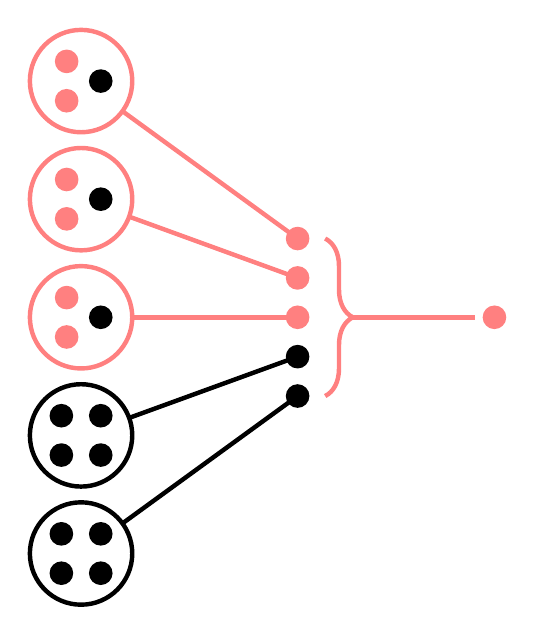
\begin{tikzpicture}[scale=0.5]

    \foreach \y in {1.5,2.5} { \fill (6, \y) circle (0.3cm); }
    \foreach \y in {3.5,4.5,5.5} { \fill[red!50] (6, \y) circle (0.3cm); }

    \draw[ultra thick] (0.5,-2.5)--(6,1.5);
    \draw[ultra thick] (0.5,0.5)--(6,2.5);
    \draw[ultra thick, red!50] (0.5,3.5)--(6,3.5);
    \draw[ultra thick, red!50] (0.5,6.5)--(6,4.5);
    \draw[ultra thick, red!50] (0.5,9.5)--(6,5.5);

    \fill[white] (0.5, -2.5) circle (1.3cm);
    \draw[ultra thick] (0.5, -2.5) circle (1.3cm);
    \fill (0, -3) circle (0.3cm); \fill (0, -2) circle (0.3cm);
    \fill (1, -3) circle (0.3cm); \fill (1, -2) circle (0.3cm);

    \fill[white] (0.5, 0.5) circle (1.3cm);
    \draw[ultra thick] (0.5, 0.5) circle (1.3cm);
    \fill (0, 0) circle (0.3cm); \fill (0, 1) circle (0.3cm);
    \fill (1, 0) circle (0.3cm); \fill (1, 1) circle (0.3cm);

    \fill[white] (0.5, 3.5) circle (1.3cm);
    \draw[ultra thick, red!50] (0.5, 3.5) circle (1.3cm);
    \fill[red!50] ({1 - sqrt(3)/2}, 3) circle (0.3cm); \fill[red!50] ({1 - sqrt(3)/2}, 4) circle (0.3cm); \fill (1, 3.5) circle (0.3cm);

    \fill[white] (0.5, 6.5) circle (1.3cm);
    \draw[ultra thick, red!50] (0.5, 6.5) circle (1.3cm);
    \fill[red!50] ({1 - sqrt(3)/2}, 6) circle (0.3cm); \fill[red!50] ({1 - sqrt(3)/2}, 7) circle (0.3cm); \fill (1, 6.5) circle (0.3cm);

    \fill[white] (0.5, 9.5) circle (1.3cm);
    \draw[ultra thick, red!50] (0.5, 9.5) circle (1.3cm);
    \fill[red!50] ({1 - sqrt(3)/2}, 9) circle (0.3cm); \fill[red!50] ({1 - sqrt(3)/2}, 10) circle (0.3cm); \fill (1, 9.5) circle (0.3cm);

    \draw [ultra thick, red!50, decorate, decoration={brace,amplitude=10pt,mirror}] (6.7,1.5) -- (6.7,5.5);
    \fill[red!50] (11,3.5) circle (0.3cm);
    \draw[ultra thick, red!50] (7.3,3.5)--(10.5,3.5);
  \end{tikzpicture}
  \caption {
    An example of $n = 17$ legislators with a minimum comittee size of $\ell=3$,
    which demonstrates that $a_3(17) \leq 6$.
  }
\end{figure}

\begin{question}
  What is an efficient way to compute $a_\ell(n)$ for general $\ell$ and $n$?
\end{question}
\begin{related}
  \item What if the president gets to choose who is on each committee but the
    opposition party gets to choose the committee size? Vice versa?
  \item What if $k_1 \leq k_2 \leq \hdots \leq k_T$? Or $k_1 \geq k_2 \geq \hdots \geq k_T$?
  \item What if ties go to the president? To the opposition?
\end{related}
\begin{references}
  \item https://oeis.org/A290323
  \item https://math.stackexchange.com/q/2395044/121988
\end{references}
\end{document}
